\chapter{Eliminación de palabras}

El proceso de relacionar las palabras migrantes con campos semánticos y eventos históricos que justifiquen su aparición, permitió establecer un forma para cuantificar la influencia entre idiomas llamada uso. Todo este método se facilitó por la eliminación de las palabras funcionales, dejando sólo palabras de contenido, pero ¿cómo se modificaría el uso entre idiomas si se eliminaran otro tipo de palabras, sin importar si estás son de contenido?

Para responder esta pregunta, se ha elaborado un nuevo algoritmo que reduce el conjunto de las palabras migrantes, y  obtiene nuevos valores para el uso entre idiomas.  Elegidos una pareja de idioma origen \textit{A} e idioma receptor \textit{B}, el proceso es el siguiente. 


\begin{enumerate}
	
	\item Se toma la lista de los préstamos acumulados de \textit{A} en \textit{B},  este corpus se denotará como \textbf{conjunto original}.
	
	\item Se escogen de forma aleatoria un grupo de letras (desde una hasta diez), y se descartan del conjunto original a aquellas  palabras cuya primer letra sea alguna de las elegidas. El nuevo corpus se denotará como \textbf{conjunto reducido}.
	
	\item Se establece un corpus  designado como \textbf{conjunto residuo}, conformado por todas las palabras eliminadas del conjunto original.  La unión del reducido y el residuo es el original. 
	
	\item En los tres conjuntos se emplea la ecuación \ref{ec.fuso}, para encontrar el uso de \textit{A} en \textit{B}. 	
	
\end{enumerate}

La intención de este método  no es eliminar a todas las palabras migrantes, sino el reducirlas  para  comparar el uso entre el conjunto original y el reducido.  Para determinar que tanto ha cambiado el uso en los dos conjuntos, se utilizará el coeficiente de determinación $R^{2}$. 

El primer criterio importante será al tomar el uso en el conjunto original como verdadero (ya que con el se establecieron los resultados del capítulo anterior),  donde sus valores para un tiempo $t$ se expresan como $O_{t}$. Si en el conjunto reducido  $v_{t}$ es el uso para el mismo $t$, mientras que  $\bar{v}$ es el promedio de todos los valores de uso, entonces  el coeficiente de determinación queda definido como:

\begin{equation}
\label{ec.dif_uso}
R^{2} = 1 - \sum_{t} \frac{ \left( v_{t}- O_{t} \right)^{2}  }{ \left( v_{t} - \bar{v} \right)^{2} }.
\end{equation}

Se empleará el concepto \textbf{conservación del uso} para aquellos idiomas cuyo uso no cambie en un intervalo de tiempo $\Delta t$. La conservación es favorable si $R^{2}$ es próximo a 1. 
%Si la conservación no es favorable, las palabras eliminadas son las más relevantes para las migraciones de \textit{A} en \textit{B}.

\section{Características de las eliminaciones}

El procedimiento de eliminar palabras, obteniendo el uso y el coeficiente de determinación, se realizó cien mil veces, cinco mil por cada pareja de idiomas.

Tras las eliminaciones, se graficaron algunos casos obtenidos, representando con un trazo continuo al uso en el conjunto original, mientras que el uso en el conjunto reducido es una serie de puntos.

Despumes de analizar las graficas de cada pareja de idiomas, se concluyó  que el uso en ambos conjuntos, cumple alguna de las siguientes características.


\begin{itemize}
	
	\item Valores iguales. Punto a punto, el uso en ambos conjuntos es el mismo. En este caso, el uso se conserva ya que las graficas son indistinguibles (figura~\ref{fig.OM1}).
	
	\item Diferencia de alturas. Punto a punto, existe una diferencia casi constante entre ambos valores de uso. En este caso, el uso también se conserva, ya que las graficas son iguales sólo que están desfasadas (figura~\ref{fig.OM2}).  
	
	\item Alteraciones por periodos. El uso en ambos conjuntos es completamente diferentes en algunos periodos de tiempo. En este caso, el uso no se conserva, ya que la graficas son diferentes (figura~\ref{fig.OM3}).

\end{itemize}



%Para ilustrar las caracterizaras mencionadas, se exponen algunas graficas obtenidas, representado con un trazo continuo al uso del conjunto original, mientras que el uso en el conjunto reducido  es una serie de puntos.   Ya que los valores en el conjunto residuo son muy pequeños, se opto por no graficarlos, para no saturar la información. 

%En cada grafica se especifican los idiomas que intervienen, así como el conjunto de letras con las cuales se hicieron las eliminaciones. 



\begin{figure}[h!]
	\centering
	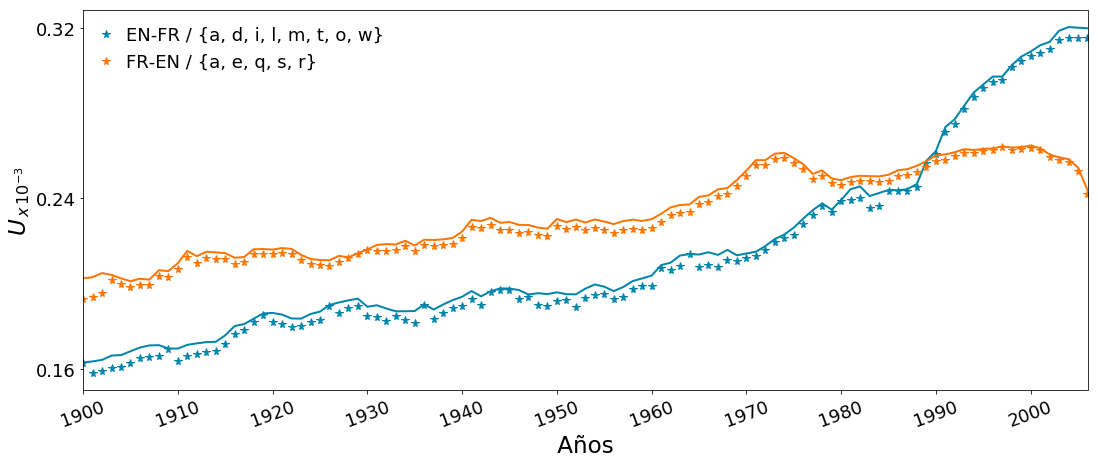
\includegraphics[scale=.375]{OM1.png}
	\caption{Eliminación de palabras en el inglés y en el francés. El uso se conserva en ambas parejas de idiomas durante todo el siglo XX, ya que $R^{2}$=0.99 para el inglés-francés y $R^{2}$=0.95 para el francés-inglés.}
	\label{fig.OM1}
\end{figure}


\begin{figure}[h!]
	\centering
	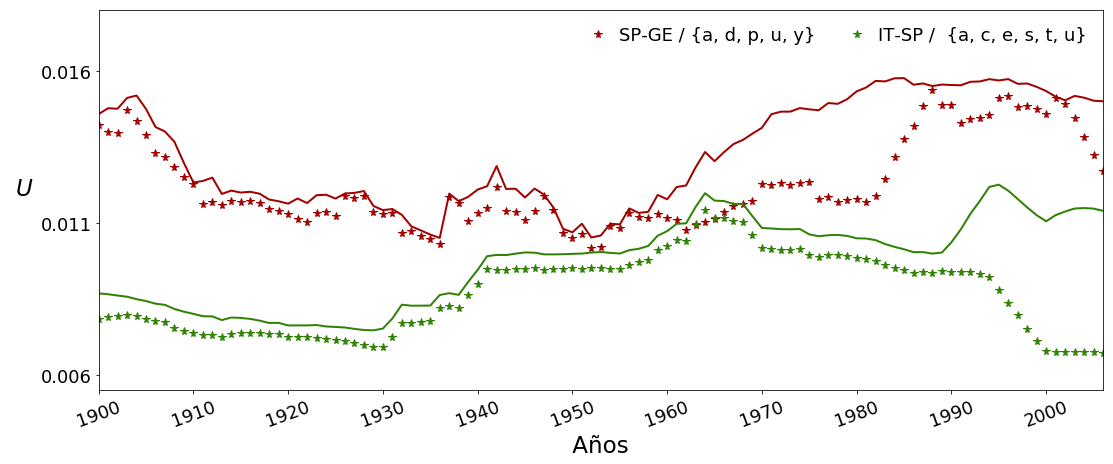
\includegraphics[scale=.375]{OM2.png}
	\caption{Eliminación de palabras en el alemán y en el italiano. El uso se conserva en ambas parejas de idiomas durante todo el siglo XX, existiendo una diferencia de alturas entre el uso original y el uso reducido.  Al despreciar la diferencia de alturas, $R^{2}$=0.86 para el alemán-inglés y $R^{2}$=0.82 para el italiano-francés.}
	\label{fig.OM2}
\end{figure}



\begin{figure}[h!]
	\centering
	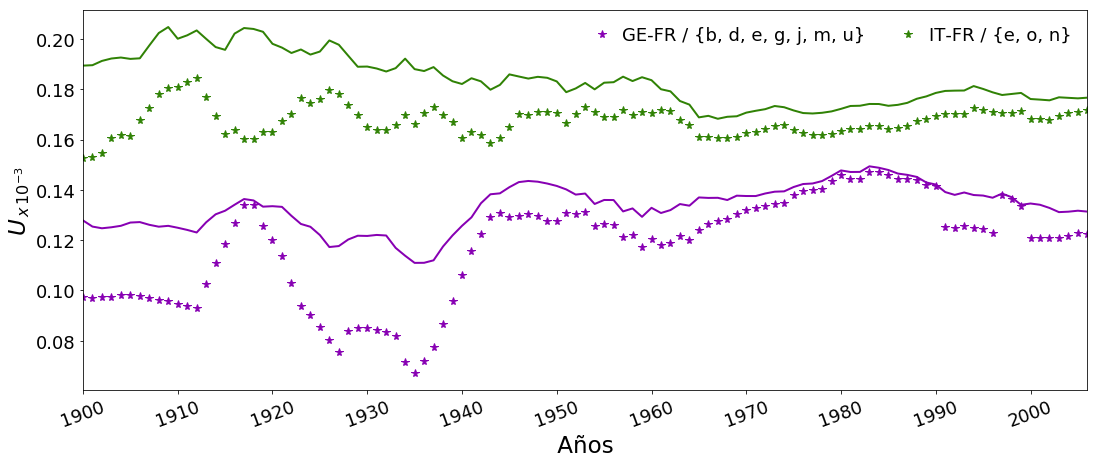
\includegraphics[scale=.375]{OM3.png}
	\caption{Eliminación de palabras en el español. Entre 1955 y 1985 el uso del español-alemán no se conservo, correspondiendo un valor de $R^{2}$=0.36 entre esos años.}
	\label{fig.OM3}
\end{figure}


La conservación del uso y sus características no siempre serán la mismas tras una eliminación con diferentes letras, sin embargo, es posible decir de manera general si el uso de un idioma se conserva. 

Para ello se agruparon y promediaron por cada pareja de idiomas y por cada idioma origen los valores del coeficiente de determinación, obtenidos tras las cien mil eliminaciones anteriores. Con el coeficiente de determinación promedio de cada idioma origen $\left \langle R^{2}  \right \rangle$ será posible decir si su uso se conserva.

La tabla~\ref{tab.conservacion} muestra por cada idioma origen,  el valor  $\left \langle R^{2}  \right \rangle$ correspondiente, así como  en cuales idiomas receptores la conservación fue mayor $R^{2}_{max}$ y menor $R^{2}_{min}$.  

De esta tabla se puede ver que la conservación del uso es menor, en las combinaciones donde el alemán este presente, ya sea como idioma origen o como idioma receptor. No obstante, en los demás idiomas la conservación del uso fue favorable, por lo que se puede decir que los idiomas conservan su uso, sin importar  cuales sean las palabras que conformen a las migraciones. 


 

%Con estos resultados se puede decir que el uso entre idiomas, no es afectado por reducir la cantidad de palabras que conforman a las migraciones,   


\begin{table}
	\centering
	\begin{tabular}{cccc}
		\textbf{} & \textbf{$\left \langle R^{2} \right \rangle$} & \textbf{$R^{2}_{max}$} & \textbf{$R^{2}_{min}$} \\
		\textbf{inglés}   & 0.85 $\pm$ 0.14   &  IT 0.97 $\pm$ 0.01  & GE 0.77 $\pm$ 0.03  \\
		\textbf{francés}  & 0.83 $\pm$ 0.12   &  EN 0.95 $\pm$ 0.02  & GE 0.66 $\pm$ 0.02  \\
		\textbf{alemán}   & 0.75 $\pm$ 0.06   &  EN 0.80 $\pm$ 0.06  & SP 0.51 $\pm$ 0.33  \\
		\textbf{italiano} & 0.87 $\pm$ 0.14   &  FR 0.93 $\pm$ 0.08  & GE 0.68 $\pm$ 0.03  \\
		\textbf{español}  & 0.88 $\pm$ 0.05   &  IT 0.94 $\pm$ 0.06  & GE 0.71 $\pm$ 0.01                                                               
	\end{tabular}
	\caption{Conservación del uso de los idiomas. El español es el idioma que es menos afectado por las eliminaciones y que conserva más su uso en los demás, seguido del italiano, el inglés, el francés y por ultimo el alemán.}
	\label{tab.conservacion}
\end{table}





\section{Resultados generales}

El realizar diferentes elecciones para reducir la cantidad de palabras migrantes, mostró la propiedad del uso entre idiomas es la misma, sin importar cuales elementos conforman el conjunto.

Individualmente. los valores de uso de una única palabra pueden ser distintos a los de otra palabra, sin embargo al tratar a todo el conjunto, el uso se comporta de la misma manera, sin importar los valores individuales de los elementos que lo conforman. 

A pesar de haber errores en el algoritmo que clasifica a los idiomas orígenes y a las palabras que migran de ellos a los demás receptores, con los resultados anteriores, se puede argumentar que no importa si se minimizan o eliminan las palabras mal clasificadas, en términos numéricos, el uso de un idioma otro va a ser el mismo.  

